\documentclass{article}

% Math
\usepackage{amsmath, amssymb, amsthm}

% Tables
\usepackage{booktabs}
\usepackage{tabularx}

% Figures
\usepackage{graphicx}
\usepackage{subcaption}

% Commands
\newcommand{\algorithmicbreak}{\textbf{break}}
\newcommand{\BREAK}{\STATE \algorithmicbreak}

% Misc
\usepackage{enumerate}
\usepackage{hyperref}
\usepackage{float}
\usepackage{algorithm}
\usepackage{algpseudocode}
\usepackage{biblatex}

\title{Econ 527 HW3}
\author{Camille Bergeron}
\date{May 2026}

\begin{document}
\maketitle

% ============================================================
\section{Speeding up VFI}
% ============================================================

This problem takes the same form as the previous problem set. We seek to solve a simple representative agent neoclassical growth model where an agent solves

\begin{equation*}
\begin{aligned}
     \max_{\{c_t\}_{t=0}^{\infty}} \mathbb{E}_0 \sum_{t=0}^{\infty} \beta^t u(c_t) \\
\text{s.t.} \quad k_{t+1} = Ak_t^{\alpha} + (1-\delta)k_t - c_t
\end{aligned}
\end{equation*}

where $u(c) = \log(c)$, $k_t > 0$, and $k_0$ is given. The problem \eqref{eq:value_fxn} can be written as the value function

\begin{equation}\label{eq:value_fxn}
    V(k) = \max_{k^{\prime} \geq 0} \log\!\left(Ak^\alpha + (1-\delta)k - k^{\prime}\right) + \beta V\!\left(k^{\prime}\right)
\end{equation}

We set the following parameters: $\beta = 0.96$, $A = 1$, $\delta = 1$, and $\alpha = 0.35$.

% ------------------------------------------------------------
\subsection{Howard Policy Iteration}
% ------------------------------------------------------------

To speed up Value Function Iteration, we implement the Howard Policy Iteration algorithm.


The results are shown in Table~\ref{tab:HPI}.

\begin{table}[H]
    \centering
    \begin{tabular}{c|c|c}
      \textbf{M} & \textbf{Time (s)} & \textbf{Bellman Iterations} \\
        \hline
        5  & 9.40  & 34 \\
        10 & 7.97  & 23 \\
        20 & 7.15  & 15
    \end{tabular}
    \caption{Results from Howard Policy Iteration}
    \label{tab:HPI}
\end{table}

where $M$ is defined as the number of policy iterations. 

% ------------------------------------------------------------
\subsection{Endogenous Grid Method}
% ------------------------------------------------------------

For the Endogenous Grid Method, it took \textbf{2433} iterations and \textbf{1.43} seconds.

% ============================================================
\section{The Stationary Distribution of State Variables}
% ============================================================

% ------------------------------------------------------------
\subsection{Net Demand Using Interpolation}
% ------------------------------------------------------------

The transition matrix was calculated via cubic spline interpolation. Using the wealth grid from the Endogenous Grid Method, cubic spline interpolants were calculated to fit a finer wealth grid (defined as 1,000 evenly spaced grid points over the range $[a_{\min}, a_{\max}]$) onto the policy grid to approximate the policy function $g(a_i, z_j)$.

Given the policy function $g(a_i, z_j)$ and the transition matrix of $z$, the pair $(a, z)$ follows a Markov process with transition matrix $\Upsilon$ of dimensions $ij \times ij$. The stationary distribution is then calculated using the eigenvalue method such that

\begin{equation}\label{eq:station}
    \Upsilon^\top \phi(a_i, z_j) = \phi(a_i, z_j)
\end{equation}

and $\sum_{i} \phi_i = 1$, where $\phi(a_i, z_j)$ is the stationary distribution with dimensions $ij \times 1$. The stationary distribution is the unit left eigenvector of $\Upsilon$, normalized to sum to one. Uniqueness is then verified.

\begin{figure}[H]
    \centering
    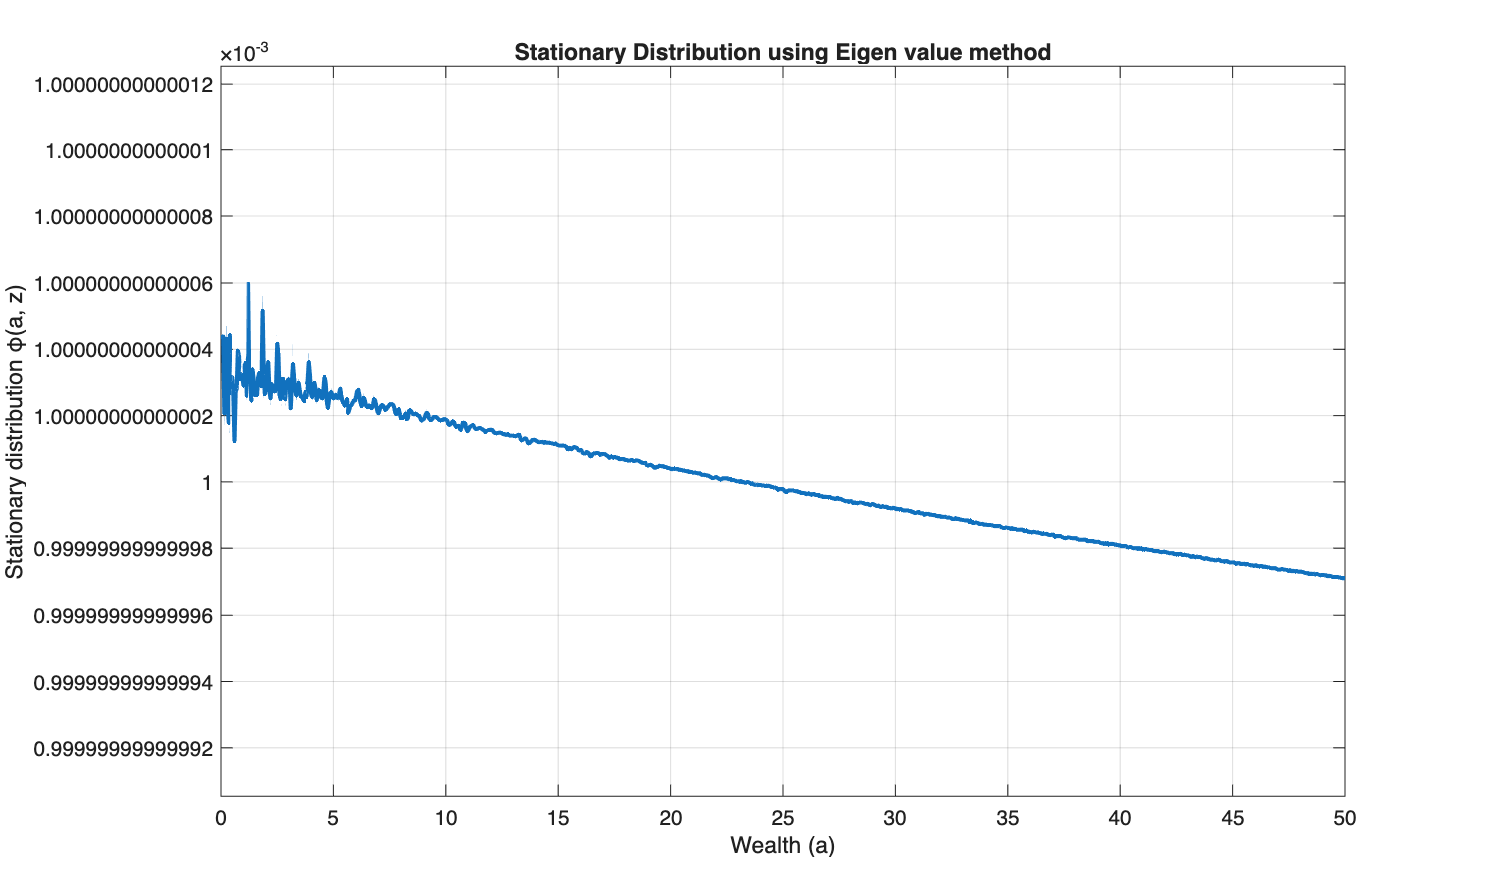
\includegraphics[width=0.75\linewidth]{../programs/figs/stationary_eigen.png}
    \caption{Stationary distribution of state variables vs.\ wealth}
    \label{fig:stationary_vs_wealth}
\end{figure}

This stationary distribution is unique and took $3.46$ seconds to compute. The net demand for assets is $-2.4999 \times 10^7 \approx 0$.

% ------------------------------------------------------------
\subsection{Net Demand Using Simulation}
% ------------------------------------------------------------

The net demand for assets using this method is $0.0017$ and took $28.96$ seconds.

% ============================================================
\section{Description of Code}
% ============================================================

Please run \texttt{PS3\_run.m}. The code is formatted so that the computer does not need to re-simulate every time; instead it loads previously generated and saved results. To see the code run from scratch (without loading saved results), delete the \texttt{results} folder found in \texttt{./programs/}. A PDF (and \texttt{.tex}) version of the output is also included (\texttt{PS3\_run.pdf}).

% ------------------------------------------------------------
\subsection{Main}
% ------------------------------------------------------------

\vspace{0.5cm}
\begin{tabularx}{\linewidth}{|X|X|X|}
    \hline
    \textbf{File} & \textbf{Description} & \textbf{Dependencies} \\
    \hline
    \texttt{PS3\_run.m} & Run file for the problem set
        & \texttt{PS3\_Q1\_HPI.m}, \texttt{PS3\_Q1\_EGM.m}, \texttt{PS3\_Q2.m} \\
    \hline
    \texttt{PS3\_run.pdf} & PDF output of \texttt{PS3\_run.m}
        & \texttt{PS3\_run.m} \\
    \hline
    \texttt{PS3.pdf} & Problem set & \\
    \hline
\end{tabularx}

% ------------------------------------------------------------
\subsection{Question 1: Howard Policy Iteration}
% ------------------------------------------------------------

\vspace{0.5cm}
\begin{tabularx}{\linewidth}{|X|X|X|}
    \hline
    \textbf{File} & \textbf{Description} & \textbf{Dependencies} \\
    \hline
    \texttt{PS3\_Q1\_HPI.m} & Sets up parameters for VFI and implements Howard Policy Iteration for $M \in \{5, 10, 20\}$
        & \texttt{rouwenhorst.m}, \texttt{polynomial\_grid.m}, \texttt{howard\_policy\_improvement.m} \\
    \hline
    \texttt{howard\_policy\_improvement.m} &
        Runs Howard policy improvement algorithm to solve for value and policy functions; iteratively updates value function using fixed-policy iteration before returning to the VFI loop
        & \texttt{VFI\_calc.m}, \texttt{policy\_calc.m} \\
    \hline
    \texttt{VFI\_calc.m} &
        Solves the Bellman equation for each $(a_i, z_j)$ pair to obtain updated value and policy grids
        & \texttt{cubic\_spline\_interpolation.m} \\
    \hline
    \texttt{policy\_calc.m} &
        Policy function iteration: updates the value grid $V^{n+1}$ and policy grid $a'$ for each $(a_i, z_j)$ pair
        & \texttt{cubic\_spline\_interpolation.m} \\
    \hline
\end{tabularx}

% ------------------------------------------------------------
\subsection{Question 1: Endogenous Grid Method}
% ------------------------------------------------------------

\vspace{0.5cm}
\begin{tabularx}{\linewidth}{|X|X|X|}
    \hline
    \textbf{File} & \textbf{Description} & \textbf{Dependencies} \\
    \hline
    \texttt{PS3\_Q1\_EGM.m} &
        Sets up parameters and implements the Endogenous Grid Method
        & \texttt{rouwenhorst.m}, \texttt{polynomial\_grid.m}, \texttt{compute\_EGM.m}, \texttt{calc\_unconstrained.m}, \texttt{calc\_constrained.m}, \texttt{cubic\_spline\_interpolation.m} \\
    \hline
    \texttt{compute\_EGM.m} &
        EGM backward step: given the exogenous grid $a'$ and marginal utility grid $\mu(a',z) = c(a',z)^{-\gamma}$, recovers the endogenous current-period wealth grid $a(a',z)$ by inverting the Euler equation
        & \\
    \hline
    \texttt{calc\_unconstrained.m} &
        Unconstrained EGM update: interpolates $V$ from the endogenous wealth grid back onto the fixed exogenous grid
        & \texttt{cubic\_spline\_interpolation.m} \\
    \hline
    \texttt{calc\_constrained.m} &
        Evaluates the Bellman equation for all $a_i$ under the constrained policy $a' = a_{\min}$ (borrowing limit)
        & \\
    \hline
\end{tabularx}

% ------------------------------------------------------------
\subsection{Question 2}
% ------------------------------------------------------------

\vspace{0.5cm}
\begin{tabularx}{\linewidth}{|X|X|X|}
    \hline
    \textbf{File} & \textbf{Description} & \textbf{Dependencies} \\
    \hline
    \texttt{PS3\_Q2.m} &
        Calculates the state transition matrix and stationary distribution; simulates the Markov chain and computes asset demand
        & \texttt{rouwenhorst.m}, \texttt{cubic\_spline\_interpolation.m}, \texttt{mc\_invdist.m}, \texttt{simulate\_markov.m}, \texttt{simulate\_a.m} \\
    \hline
    \texttt{simulate\_markov.m} &
        Simulates the Markov chain from the state transition matrix
        & \texttt{mc\_invdist.m} \\
    \hline
    \texttt{simulate\_a.m} &
        Simulates wealth and sets initial state to the borrowing limit
        & \\
    \hline
\end{tabularx}

% ------------------------------------------------------------
\subsection{General Functions}
% ------------------------------------------------------------

\vspace{0.5cm}
\begin{tabularx}{\linewidth}{|X|X|X|}
    \hline
    \textbf{File} & \textbf{Description} & \textbf{Dependencies} \\
    \hline
    \texttt{rouwenhorst.m} &
        Rouwenhorst's method for discretizing an AR(1) process
        & \\
    \hline
    \texttt{cubic\_spline\_interpolation.m} &
        Cubic spline interpolation between grid points
        & \\
    \hline
    \texttt{mc\_invdist.m} &
        Computes the invariant distribution of a Markov chain with transition matrix $\Pi$
        & \\
    \hline
\end{tabularx}

% ============================================================
\section{Acknowledgments}
% ============================================================

Thanks to Professor Greaney for providing essential functions and for being very helpful throughout the course.

% ============================================================
\section{AI Usage}
% ============================================================

AI (specifically Claude) was used to debug code and format \LaTeX.

\end{document}